\apendice{Documentación de usuario}

\section{Introducción}

\section{Requisitos de usuarios}

\section{Instalación}

\section{Manual del usuario}
\subsection{\textit{Alp’s Labeling Tool (ALT)}}

Para hacer el etiquetado se va a usar \textit{Alp’s Labeling Tool (ALT)}.\\
Se trata de un etiquetador bastante sencillo, tanto de descargar como de usar.\\

\subsubsection{Software necesario}
Para poder hacer uso de ella para la funcionalidad que queremos, en este caso etiquetar imágenes, vamos a neceseitar 3 tipos de software:\\
\begin{itemize}
	\item \href{http://fiji.sc/#download}{Fiji}. Esta herramienta no precisa de instalación como tal, simplemente hay que descomprimir la carpeta que contiene la aplicación y ubicarla donde nos resulte más cómoda trabajar on ella.\\
	
	Para descargarla solo es necesario escoger el sistema operativo sobre el que vamos a trabajar.
	\item \href{https://github.com/imagejan/ActionBar/releases/download/SciJava-Parameters/action_bar-2.0.5-SNAPSHOT.jar}{Action Bar}. Se trata de un plugin que hay que instalar directamente en la aplicación Fiji.
	\item \href{https://www.dropbox.com/s/ihkr0ahhif3csvp/ALT_Windows_22mar2017.zip?dl=0}{ALT}. Este macro plugin nos va ha permitir cargar las imágenes, dibujar etiquetas sobre ellas, poner nombres a dichas etiquetas, guardar la información, volver a cargarla y devolver las coordenadas en formato .txt o .csv.
\end{itemize}

Considerando que ya se tiene todo el software especificado,
la instalación de la aplicación se realizará siguiendo los siguientes pasos:
\begin{enumerate}
	\item Lo primero que vamos a hacer es descomprimir la carpeta que contiene la aplicación de \textbf{Fiji} y ubicar dicha carpeta dónde nos sea más cómodo trabajar.
	\item A continuación, descomprimimos el plugin de \textbf{Action Bar} y lo dejamos dónde lo podamos usar.
	\item Vamos a iniciar la aplicación, la cual se encuentra dentro de la carpeta extraída. Veremos una barra de tareas como la mostrada en la imagen [\ref{fig:barra_de_tareas}]
	\begin{figure}
		\centering
		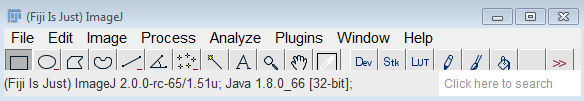
\includegraphics[width=0.7\linewidth]{img/barra}
		\caption{Barra de tareas de Fiji}
		\label{fig:barra_de_tareas}
	\end{figure}
	
	\item en la opción de menú "Plugins", vamos a seleccionar "Install Plugin..."	y tendremos que escoger el plugin "Action Bar" que habíamos descomprimido anteriormente. Tras esto reiniciamos la aplicación.
	\item Ahora abrimos la carpeta que contiene la aplicación que contiene la aplicación Fiji y abrimos el .zip que contiene ALT, la última descarga que hemos hecho. 
	\item Dentro del .zip de ALT hay una carpeta llamada "plugins". La seleccionamos y la arrastramos dentro de la carpeta de la aplicación.
	\item Reiniciar la aplicación en el caso de que estuviera abierta.
\end{enumerate}
Todo este proceso de instalación se puede ver en \href{https://www.youtube.com/watch?v=G6ib950iDvQ}{videotutoriales} que el propio desarrollador ha subido a Youtube.
\subsubsection{Uso de la aplicación}
\subsubsection{Recomendaciones}